
%(BEGIN_QUESTION)
% Copyright 2010, Tony R. Kuphaldt, released under the Creative Commons Attribution License (v 1.0)
% This means you may do almost anything with this work of mine, so long as you give me proper credit

FOUNDATION Fieldbus H1 cable is comprised of two ungrounded conductors surrounded by a grounded shield.  Coupling devices provide easy connection points for new devices on the network segment:

$$\includegraphics[width=15.5cm]{i04574x01.eps}$$

\vskip 10pt

Suppose the H1 segment shown above is newly-constructed, and you are asked to perform some basic tests on the cable to ensure there are no major problems before it is energized for the first time.  Describe a simple way for you to electrically test the whole length of the segment ``trunk'' for open or short faults in as few steps as possible.

\vskip 20pt \vbox{\hrule \hbox{\strut \vrule{} {\bf Suggestions for Socratic discussion} \vrule} \hrule}

\begin{itemize}
\item{} Suppose a design engineer from a test and measurement company approached you to learn more about FOUNDATION Fieldbus, in order to design a cable tester specifically for testing H1 segments.  What tests should such a tester automatically perform, and how exactly would it do so?
\item{} Suppose all the cabling in the segment shown above is Type C cable according to the Fieldbus standard.  How much length will be allowed in this network, and where is that length measured?
\end{itemize}

\underbar{file i04574}
%(END_QUESTION)





%(BEGIN_ANSWER)

Hint: connect an ohmmeter to the two cable conductors at the host end while a fellow technician removes the far terminator and stands ready with a jumper wire and a hand-held radio (to communicate with you).

%(END_ANSWER)





%(BEGIN_NOTES)

Measure resistance (ohms) with the ``trunk'' cable open at the far end, then again with a direct short at the far end (where the terminator used to connect).  These two readings will confirm continuity and the absence (or presence) of internal shorts.

%INDEX% Fieldbus, FOUNDATION (H1): segment troubleshooting

%(END_NOTES)

